\documentclass{beamer}

\usepackage[utf8]{inputenc}%uso utf8 invece di utf8x per poter mettere gli accenti nel titolo del pdf. Questo mi crea problemi con i °
\usepackage{default}
\usepackage[italian]{babel}
\usepackage{graphicx}
\usepackage[version=3]{mhchem} % Formula subscripts using \ce{}
\usepackage{booktabs}
\usepackage{color}
\usepackage{textcomp}%risolvo il problema col ° usando \textdegree e questo pacchetto


\usetheme{Warsaw}        % layout complessivo. 
\useinnertheme{default} % layout interno.
\useoutertheme{default} % layout esterno.
\usecolortheme{wolverine} % schema di colori.
\usefonttheme{default}  % schema dei font.

\hypersetup{pdfauthor={Ilario Gelmetti},pdfsubject={Synthesis and Reactivity of Silylformylation Products Derived from Terminal Alkynes},pdfkeywords={Alkynes, silanes, silylformylation, organic chemistry, organometallics, rearrangement, carbonylation, lactams, lactons, aldehydes, silylcarbocyclisation, desilylation, alpha-beta-unsaturated aldehydes, supported rhodium nanoparticles, metal vapour synthesis, catalysis},pdftitle={Sintesi e reattività dei prodotti di sililformilazione derivati da alchini terminali}}


\setbeamertemplate{navigation symbols}{} %per eliminare i bottoni della barra di navigazione in basso a destra
\AtBeginSection[]{\frame{\tableofcontents[current,hideothersubsections]}}
\newcommand{\diapo}[1]{\subsection{#1}\begin{frame}\frametitle{#1}}


\title[Sintesi e reattività dei prodotti di sililformilazione di alchini]{Sintesi e reattività dei prodotti di sililformilazione derivati da alchini terminali}
\author{Ilario Gelmetti}
\institute{Scuola Normale Superiore di Pisa}
\date{20 maggio 2011}
\logo{
\includegraphics[width=0.07\paperwidth]{img/snslogo.png}}

\begin{document}
\begin{frame}
  \titlepage
\end{frame}

\setbeamertemplate{footline}{%
\leavevmode\hbox{%
\begin{beamercolorbox}[wd=.2\paperwidth,ht=2.5ex,dp=1.125ex,leftskip=.3cm plus1fill,rightskip=.3cm]{author in head/foot}%
\usebeamerfont{author in head/foot}\insertshortauthor
\end{beamercolorbox}%
\begin{beamercolorbox}[wd=.6\paperwidth,ht=2.5ex,dp=1.125ex,leftskip=1.1cm,rightskip=.3cm plus1fil]{title in head/foot}%
\usebeamerfont{title in head/foot}\insertshorttitle
\end{beamercolorbox}%
\begin{beamercolorbox}[wd=.2\paperwidth,ht=2.5ex,dp=1.125ex,leftskip=0.3cm,rightskip=.3cm plus1fil]{author in head/foot}%
\usebeamerfont{author in head/foot}\insertframenumber /28
\end{beamercolorbox}}%
\vskip0pt%
}

\section{Introduzione}
\diapo{La chimica del silicio}
Il silicio come ``{\bf traghettatore}'': 
$$\ce{R ->[?] P}$$
$$\ce{R ->C[+Si] I ->[-\ce{Si}] P}$$
\pause
I {\bf legami del silicio}:
\begin{itemize}
 \item {\bf facile rottura} eterolitica da parte di reagenti ionici, {\bf ossigeno e alogeni};
 \item se {\bf legato al carbonio} può essere considerato un {\bf super-protone};
 \item se {\bf legato all'ossigeno} può essere considerato un {\bf protone indebolito}.
\end{itemize}
\end{frame}


%%%%%%%%%%%%%%%%%%%%%%%%%%%%%%%%%%%%%%%%%%%%%%%%%%%%%%%%%%%%%%%%%%%%
\logo{}

\begin{frame}
\frametitle{La chimica del silicio}
\begin{block}{Effetto $\beta$: ($\sigma$--p)$_\pi$}
\begin{figure}{\centering{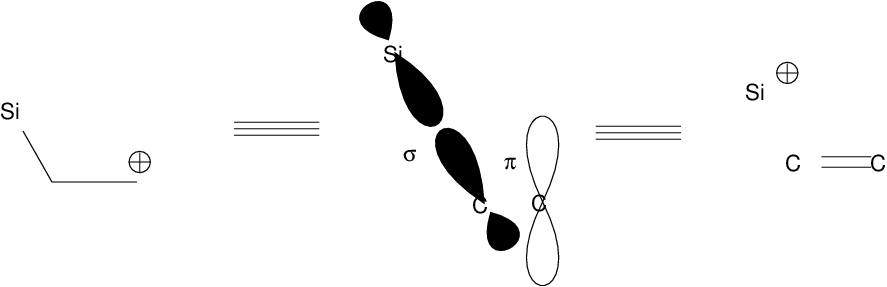
\includegraphics[width=0.7\textwidth]{img/intro/b-effect.png}}}\end{figure}
\end{block}
\pause
\begin{block}{$\alpha$ anioni: ($\sigma$*--p)$_\pi$}
\begin{figure}{\centering{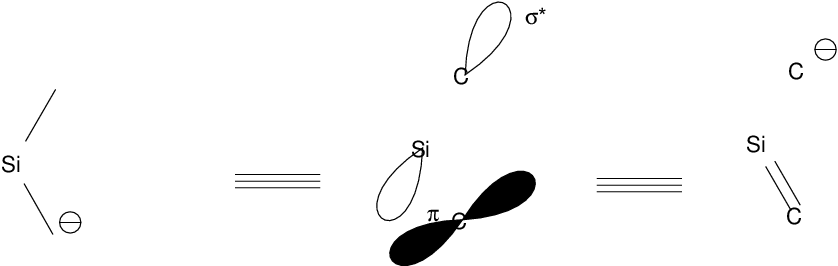
\includegraphics[width=0.7\textwidth]{img/intro/a-anions.png}}}\end{figure}
\end{block}
\end{frame}

\logo{
\includegraphics[width=0.07\paperwidth]{img/snslogo.png}}

%%%%%%%%%%%%%%%%%%%%%%%%%%%%%%%%%%%%%%%%%%%%%%%%%%%%%%%%%%%%%%%%%%%%

\diapo{Schema generale delle reazioni di interesse}
\begin{figure}{\centering{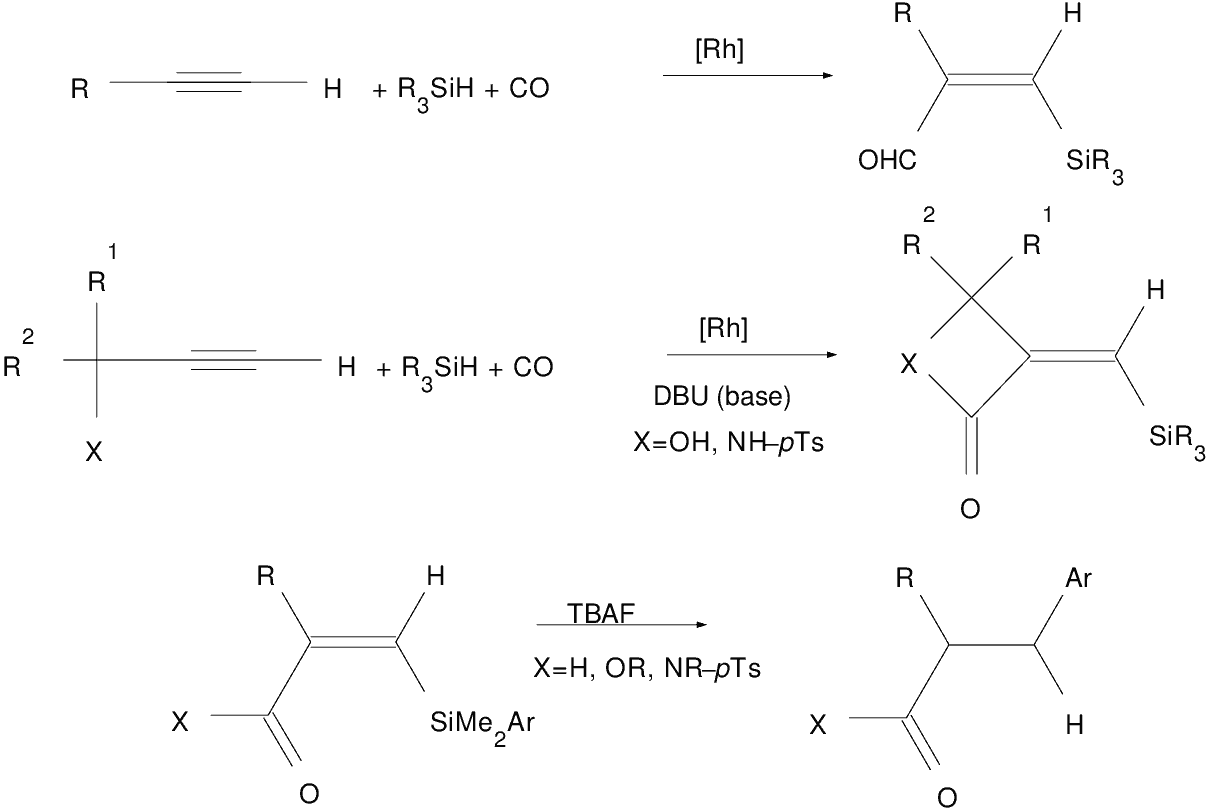
\includegraphics[width=0.8\textwidth]{img/intro/generale.png}}}\end{figure}


\end{frame}

\subsection{Prodotti ottenibili da $\beta$-silil alchenali}\begin{frame}\frametitle{Prodotti ottenibili da $\beta$-silil alchenali}
I $\beta$-sililalchenali ottenuti possono poi essere trasformati sfruttando la {\bf reattività sia di un carbonile $\alpha , \beta $ insaturo sia di un vinil silano}.
\begin{figure}{\centering{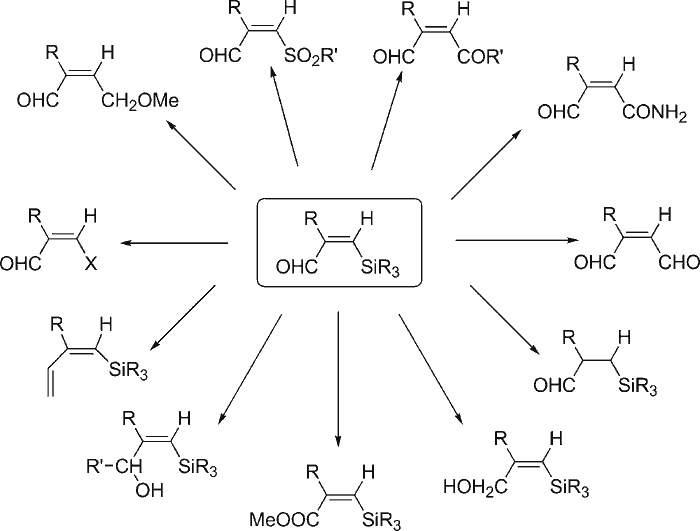
\includegraphics[width=0.6\textwidth]{img/intro/altri_prodotti_ottenibili.png}}}\end{figure}


\end{frame}


%%%%%%%%%%%%%%%%%%%%%%%%%%%%%%%%%%%%%%%%%%%%%%%%%%%%%%%%%%%%%%%%%%%%



\section{La sililformilazione di alchini e la desililazione}

\diapo{Idrosililazione di alchini}
L'{\bf idrosililazione} di alchini terminali catalizzata da acido cloroplatinico è {\bf regioselettiva e diastereoselettiva} come mostrato in figura.
\begin{figure}{\centering{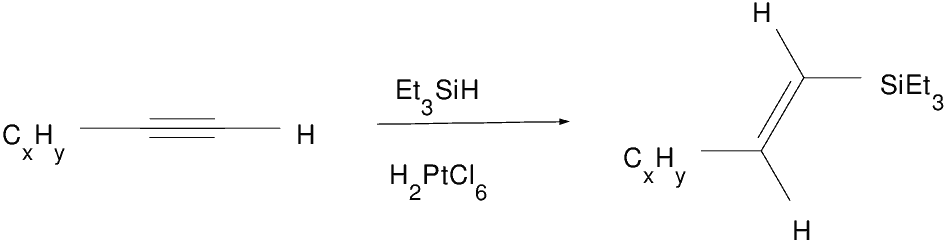
\includegraphics[width=0.80\textwidth]{img/sintesi/idro2.png}}}\end{figure}


\end{frame}

%%%%%%%%%%%%%%%%%%%%%%%%%%%%%%%%%%%%%%%%%%%%%%%%%%%%%%%%%%%%%%%%%%%%ho 


\diapo{Sililformilazione di alchini}
La {\bf sililformilazione} avviene in {\bf atmosfera di CO} e con catalizzatori a base di {\bf rodio}. 

Il {\bf silicio attacca l'atomo terminale} mentre il CO attacca il carbonio interno dando un'aldeide, come mostrato in alto nella figura.
\begin{columns}
\column{0.5\linewidth}
\begin{figure}{\centering{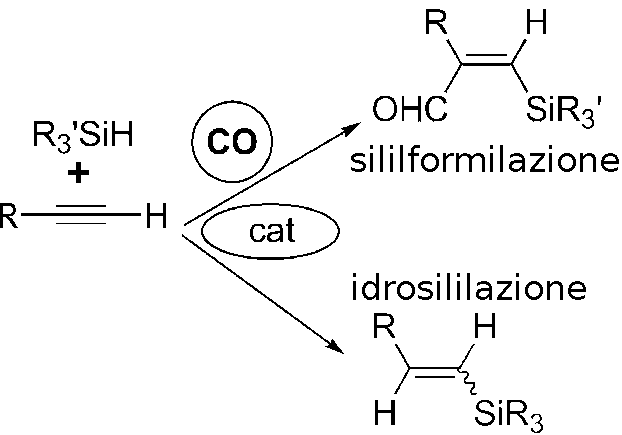
\includegraphics[width=1\textwidth]{img/sintesi/byproducts.png}}}\end{figure}
\pause
\column{0.5\linewidth} 

{\bf Se R è ingombrato} il prodotto di sililformilazione si forma {\bf più difficilmente} mentre è favorito il {\bf sottoprodotto di idrosililazione}.
\end{columns}

\end{frame}

\subsubsection{Idrosilani}\begin{frame}\frametitle{Sililformilazione di alchini}\framesubtitle{Idrosilani}
\begin{columns}
\column{0.35\linewidth}I {\bf sostituenti} sul reagente {\bf idrosilano} sono {\bf importanti} per il successo della reazione. 
\column{0.65\linewidth}\begin{figure}{\centering{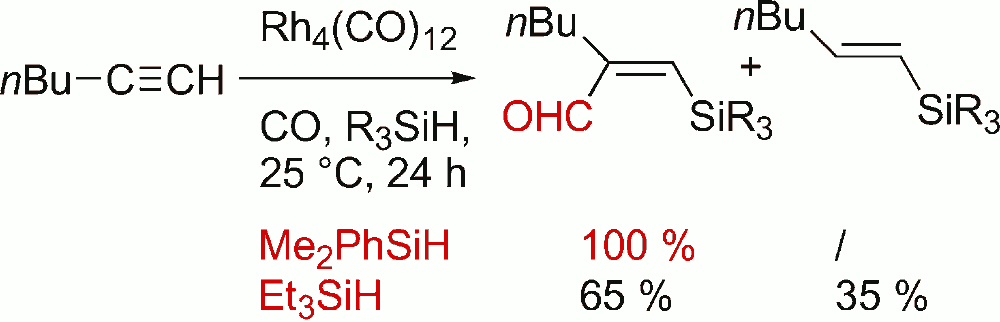
\includegraphics[width=1\textwidth]{img/sintesi/idrosilani.png}}}\end{figure}
\end{columns}\vspace{10pt}
La presenza di un sostituente {\bf aromatico favorisce} la sililformilazione rispetto all'idrosiliazione.

Sono {\bf preferibili} sostituenti aromatici con {\bf piccolo ingombro sterico}. 

\end{frame}

%%%%%%%%%%%%%%%%%%%%%%%%%%%%%%%%%%%%%%%%%%%%%%%%%%%%%%%%%%%%%%%%%%%%

\diapo{Sililcarbociclizzazione di ammine ed alcoli propargilici}
In presenza di un {\bf gruppo alcolico o di una ammide in posizione propargilica} ed impiegando una {\bf base} in quantità catalitica è possibile ottenere {\bf sililcarbociclizzazione}. 
\pause
\begin{figure}{\centering{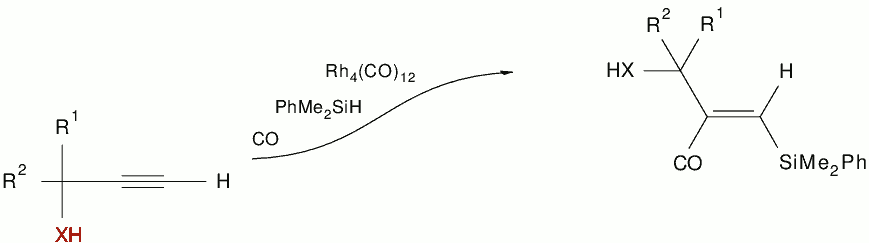
\includegraphics[width=0.6\textwidth]{img/sintesi/ciclizzaz-x1.png}}}\end{figure}
\pause
\vskip -30pt
\begin{figure}{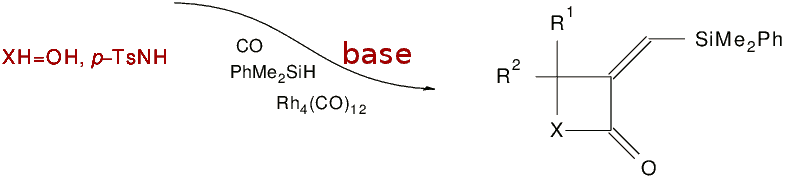
\includegraphics[width=0.75\textwidth]{img/sintesi/ciclizzaz-x2.png}}\end{figure}
\pause
Questa reattività è {\bf favorita da idrosilani con aromatici ingombrati e da \ce{R^1} e \ce{R^2} stericamente ingombranti}.

\end{frame}

%%%%%%%%%%%%%%%%%%%%%%%%%%%%%%%%%%%%%%%%%%%%%%%%%%%%%%%%%%%%%%%%%%%%
\logo{}
\diapo{Desililazione con migrazione del gruppo aromatico}

Tra tutte le numerose possibili ulteriori trasformazioni verrà esposta solamente la {\bf desililazione promossa da fluoruri con migrazione del gruppo aromatico} presente sull'idrosilano.  
\begin{figure}{\centering{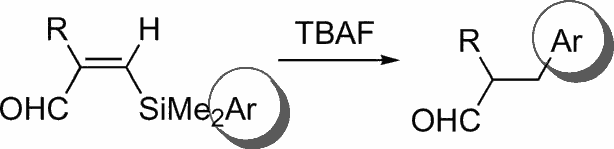
\includegraphics[width=0.5\textwidth]{img/sintesi/trasf_aromatico.png}}}\end{figure}
\pause
\begin{columns}
\column{0.8\linewidth}Inizialmente avviene l'{\bf attacco del fluoruro sull'atomo di silicio} rendendolo pentavalente. 
\pause

 Poi si ha una {\bf migrazione 1,2 anionotropica} del gruppo aromatico 
con ritenzione della configurazione originale anche in presenza di sostituenti in orto.
\column{0.3\linewidth}
\vskip -5pt
\begin{figure}{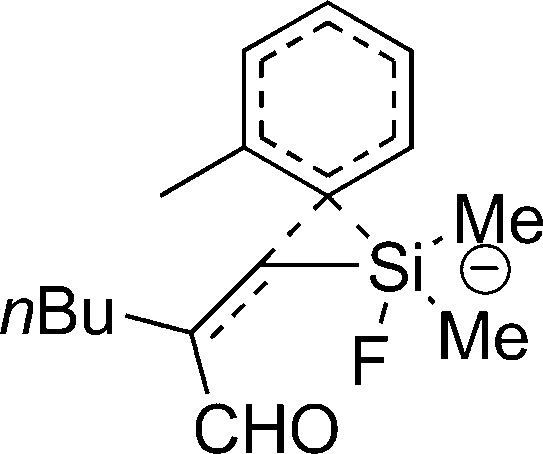
\includegraphics[width=1\textwidth]{img/sintesi/trasposizione12.png}}\end{figure}
\end{columns}
\end{frame}

%%%%%%%%%%%%%%%%%%%%%%%%%%%%%%%%%%%%%%%%%%%%%%%%%%%%%%%%%%%%%%%%%%%%

\begin{frame}\frametitle{Desililazione con migrazione del gruppo aromatico}
\begin{columns}
\column{0.5\linewidth}
Successivamente alla trasposizione 1,2 anionotropica dell'aromatico si ha una {\bf trasposizione [1,4]Si da carbonio ad ossigeno} detta ``riarrangiamento di Brook''. 

{\onslide<2>

La \emph{driving force} di questa reazione è la {\bf differenza di energia di legame Si-C e Si-O}. 

Infine il sililetere viene {\bf idrolizzato ad aldeide}.}

\column{0.5\linewidth}{\onslide<1,2>\begin{figure}{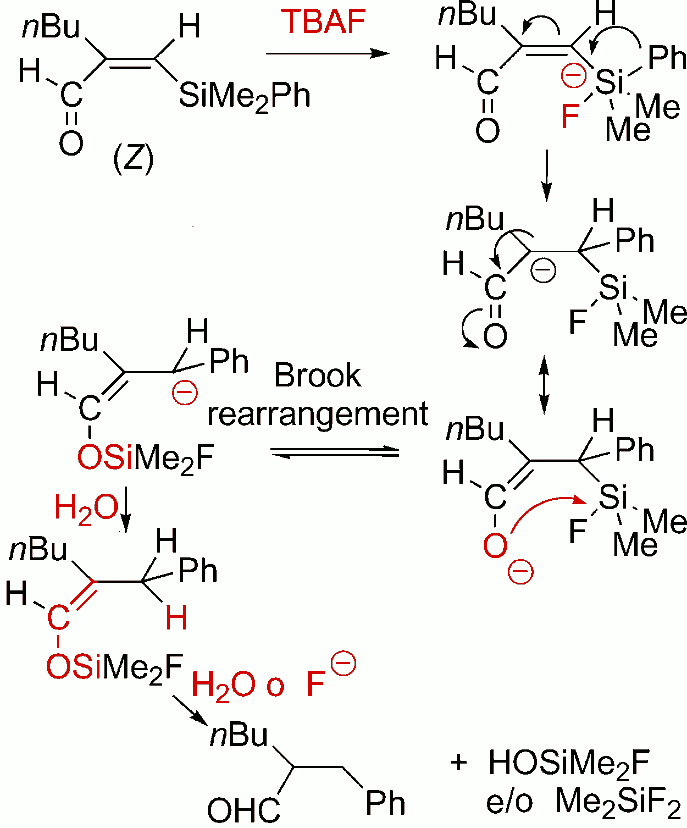
\includegraphics[width=1\textwidth]{img/sintesi/desililaz.png}}\end{figure}}
\end{columns}


\end{frame}

\logo{
\includegraphics[width=0.07\paperwidth]{img/snslogo.png}}

\section{Catalisi delle reazioni}
\diapo{Due possibili meccanismi di reazione}
\begin{figure}{\centering{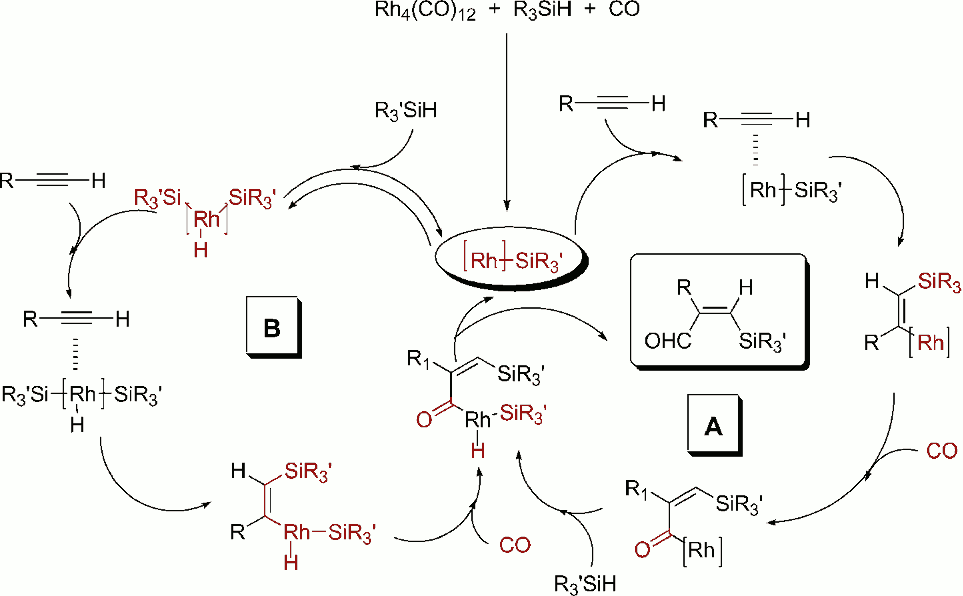
\includegraphics[width=0.9\textwidth]{img/catalisi/cicli.png}}}\end{figure}

\end{frame}
\subsubsection{Quantità di catalizzatore}\begin{frame}\frametitle{Due possibili meccanismi di reazione}\framesubtitle{Quantità di catalizzatore}
\begin{columns}
\column{0.45\linewidth}
Una {\bf eccessiva quantità di catalizzatore favorisce la idrosililazione}. 

Sembra che la grande quantità di catalizzatore renda più efficiente l'eliminazione riduttiva rispetto all'inserimento di \ce{CO}. 
\column{0.5\linewidth}\begin{figure}{\centering{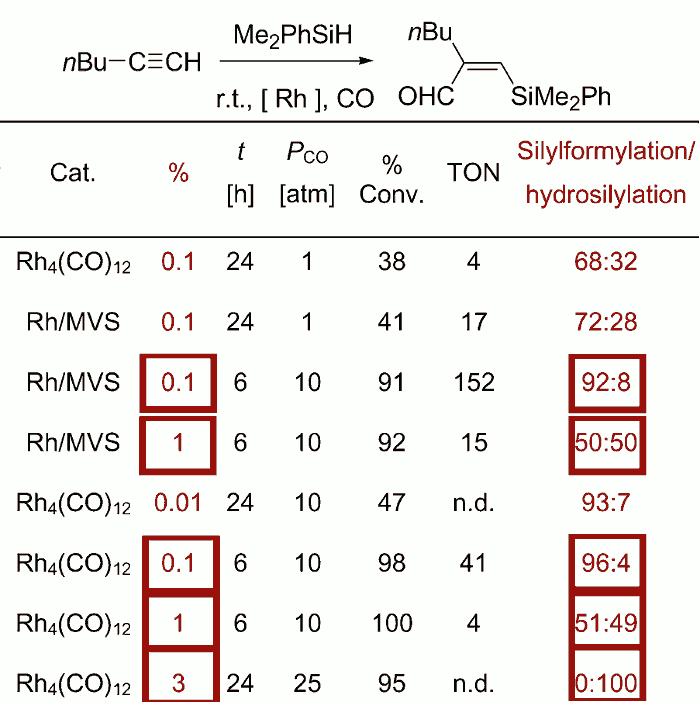
\includegraphics[width=0.9\textwidth]{img/catalisi/quantcat.png}}}\end{figure}
\end{columns}


\end{frame}
\logo{}
\diapo{Catalizzatori ``tradizionali''}
Sono stati {\bf testati numerosi catalizzatori} per la reazione di {\bf sililformilazione}:
\begin{figure}{\centering{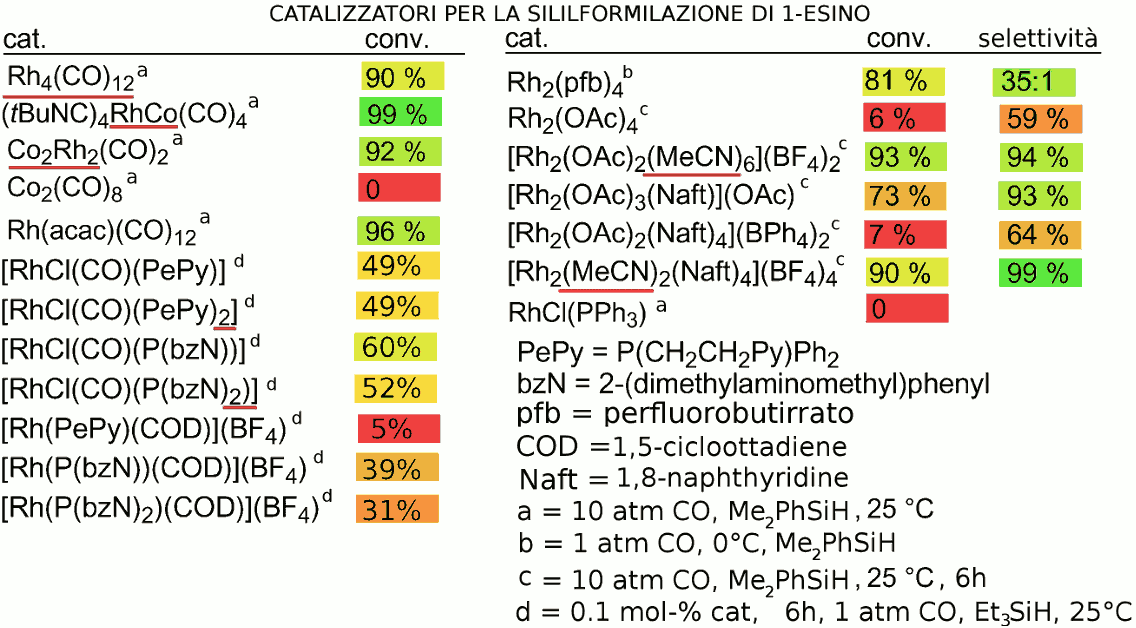
\includegraphics[width=1\textwidth]{img/catalisi/catalizzatori.png}}}\end{figure}

\end{frame}
\logo{
\includegraphics[width=0.07\paperwidth]{img/snslogo.png}}

%%%%%%%%%%%%%%%%%%%%%%%%%%%%%%%%%%%%%%%%%%%%%%%%%%%%%%%%%%%%%%%%%%%%

\diapo{Catalizzatori realizzati con MVS}
Tramite tecnica {\bf Metal Vapour Synthesis} sono stati preparati catalizzatori {\bf supportati} o nanocluster di rodio (stabili in mesitilene solo a -40\textdegree C).
\begin{figure}{\centering{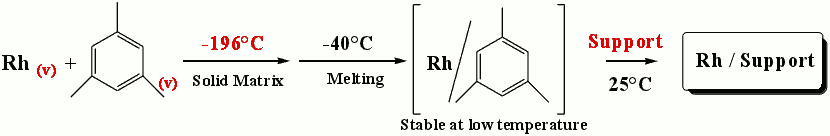
\includegraphics[width=1\textwidth]{img/catalisi/mvs.png}}}\end{figure}
Il supporto è stato utilizzato sia per avere una stabilità maggiore sia per ottenere una catalisi eterogenea. 
\pause

Purtroppo s'è riscontrato che {\bf la catalisi avviene omogenea} da parte di rodio liberatosi dal supporto.
\end{frame}
\definecolor{orange}{RGB}{255,160,0}

\subsubsection{Risultati}\begin{frame}\frametitle{Catalizzatori realizzati con MVS}\framesubtitle{Risultati}
I {\bf catalizzatori MVS danno attività specifiche maggiori} rispetto al riferimento \ce{Rh4(CO)12}.


 \pause {\bf Supporti molto polari liberano meno particelle} ed hanno efficacie minori. 
{\bf Catalizzatori supportati commerciali} hanno efficacia quasi {\bf nulla} a causa della {\bf dimensione delle nanoparticelle molto maggiore}. 
{\footnotesize\begin{center}
   \begin{tabular}{c c c}
\multicolumn{3}{c}{Sililformilazione di 1-esino} \\
\multicolumn{3}{c}{{\tiny(t=6h, 2mmol \ce{Me2OhSiH}, 2mmol 1-esino, 2$\mu$mol Rh, 2mL toluene, 25\textdegree C, 10atm CO)}} \\
 Catalizzatore & Conversione (\%) & Selettività (\%) \\
\midrule
\ce{Rh4(CO)12} & \color{green}98 & \color{green}96 \\
\ce{Rh$/$Mesitilene} & \color{yellow} 91 & \color{yellow}92 \\
\ce{Rh$/$C (MVS)} & \color{orange}81 & \color{yellow}94 \\
\ce{Rh$/$Fe2O3 (MVS)} & \color{red}43 & \color{green}97 \\
\ce{Rh$/$C (commerciale)} & \color{red}12 & \color{green}97
   \end{tabular}
  \end{center}}
\end{frame}
%%%%%%%%%%%%%%%%%%%%%%%%%%%%%%%%%%%%%%%%%%%%%%%%%%%%%%%%%%%%%%%%%%%%
\AtBeginSection[]{\frame{\tableofcontents[current,hideothersubsections,subsubsectionstyle=hide]}}

\section{Substrati usati, meccanismi di reazione e risultati sperimentali}

\subsection{Alchini funzionalizzati con alogenuri}
\subsubsection{Sililformilazione}\begin{frame}\frametitle{Alchini funzionalizzati con alogenuri}\framesubtitle{Sililformilazione}
Il risultato della {\bf sililformilazione di alchini funzionalizzati con buoni gruppi uscenti} dipende dalla posizione di questi:
\begin{itemize}
 \item sostituenti in alfa al triplo legame: si ha decomposizione; 
 \item sostituenti in posizioni più lontane non sono problematici per la sililformilazione.
\end{itemize}


\end{frame}

%%%%%%%%%%%%%%%%%%%%%%%%%%%%%%%%%%%%%%%%%%%%%%%%%%%%%%%%%%%%%%%%%%%%
\logo{}
\subsubsection{Desililazione}\begin{frame}\frametitle{Alchini funzionalizzati con alogenuri}\framesubtitle{Desililazione}
Nella {\bf desililazione con migrazione} del gruppo aromatico si ha un {\bf effetto importante} sulla reattività da parte di {\bf alogenuri e tosilati}.
\begin{columns}
\column{0.5\linewidth}


In dipendenza dalla posizione dell'alogenuro nella catena alifatica del $\beta$-sililalchenale si può avere la {\bf formazione di cicli secondo diversi meccanismi}.  
\column{0.5\linewidth}\begin{figure}{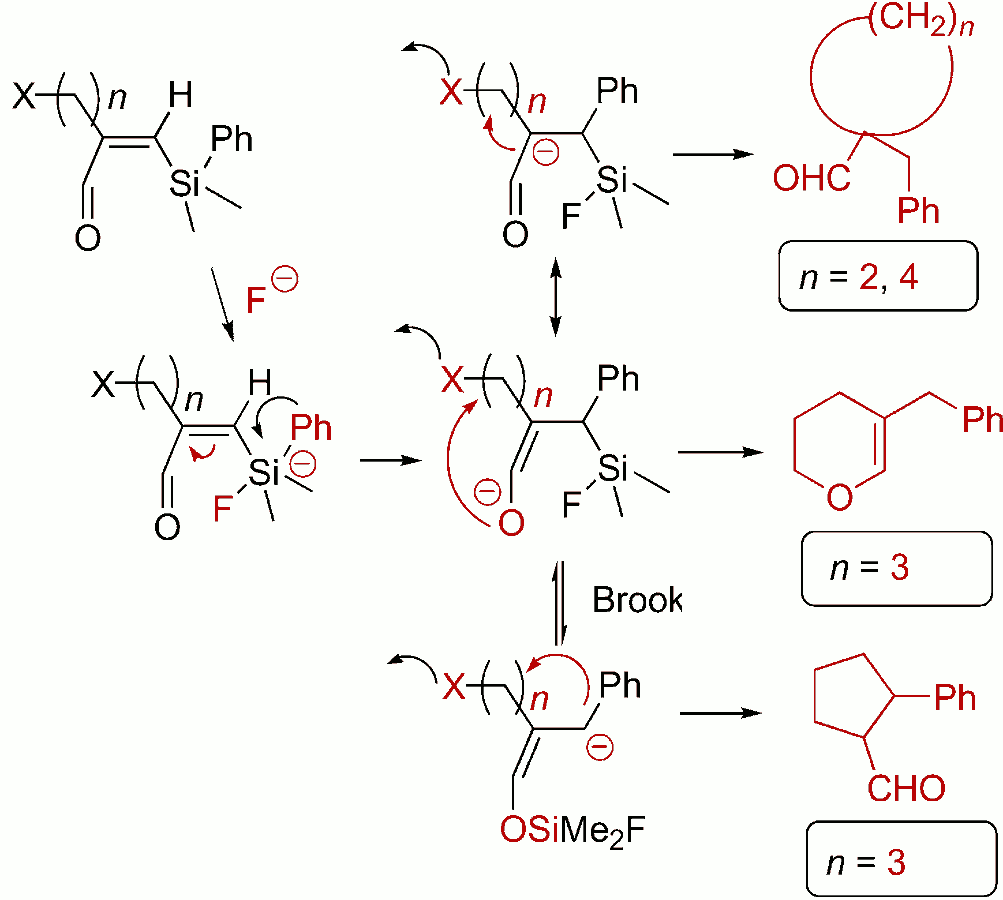
\includegraphics[width=1\textwidth]{img/substrati/alogenuri.png}}\end{figure}

\end{columns}
\end{frame}
\logo{
\includegraphics[width=0.07\paperwidth]{img/snslogo.png}}

\begin{frame}\frametitle{Alchini funzionalizzati con alogenuri}\framesubtitle{Desililazione}
Anche in presenza di gruppi uscenti non ottimi come il cloruro si ha una prevalenza della formazione di cicli sul prodotto lineare 1-benzilaldeide. {\bf In ogni caso si formano anelli a 3, 5 e 6 membri}.
 \begin{figure}{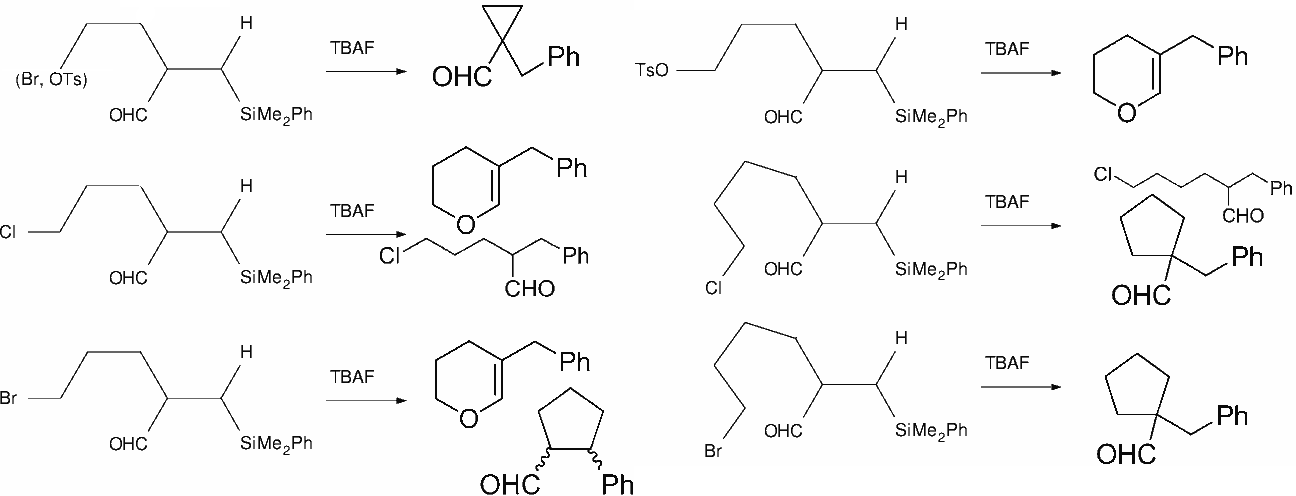
\includegraphics[width=1\textwidth]{img/substrati/alogenuri3.png}}\end{figure}

\end{frame}



%%%%%%%%%%%%%%%%%%%%%%%%%%%%%%%%%%%%%%%%%%%%%%%%%%%%%%%%%%%%%%%%%%%%

\subsection{Ammine propargiliche}
\subsubsection{Sililformilazione}\begin{frame}\frametitle{Ammine propargiliche}\framesubtitle{Sililformilazione}
La {\bf sililformilazione di ammine} propargiliche va a buon fine se l'{\bf ammina è protetta come tosilammide} (l'ammina libera potrebbe avvelenare il catalizzatore).
\begin{figure}{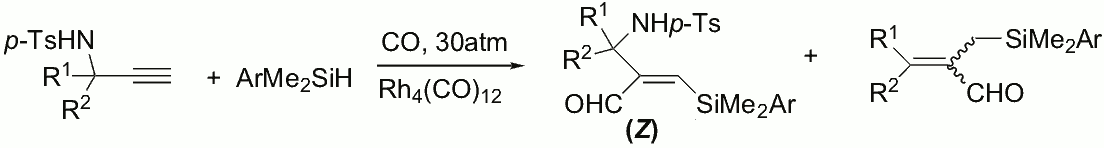
\includegraphics[width=0.95\textwidth]{img/substrati/ammine-sililform.png}}\end{figure}
Si hanno i {\bf prodotti secondari} mostrati in figura (probabilmente secondo un meccanismo in cui una seconda molecola di silano dà idrosililazione 1,4 del gruppo aldeidico nel $\beta$-sililalchenale e quindi eliminazione di una silanammide).


\end{frame}

%%%%%%%%%%%%%%%%%%%%%%%%%%%%%%%%%%%%%%%%%%%%%%%%%%%%%%%%%%%%%%%%%%%%

\subsubsection{Desililazione di $\beta$-sililalchenali}\begin{frame}\frametitle{Ammine propargiliche}\framesubtitle{Desililazione di $\beta$-sililalchenali}
\begin{columns}
\column{0.55\linewidth}
Su $\beta$-sililalchenali aventi in posizione $\alpha$ un {\bf gruppo tosilammide} (o un altro buon gruppo uscente) la desililazione avviene con {\bf eliminazione} della tosilammide per ottenere una 2-metilaril-2-alchenale.

Si ha preferenzialmente il prodotto più stabile E.

\column{0.45\linewidth}\begin{figure}{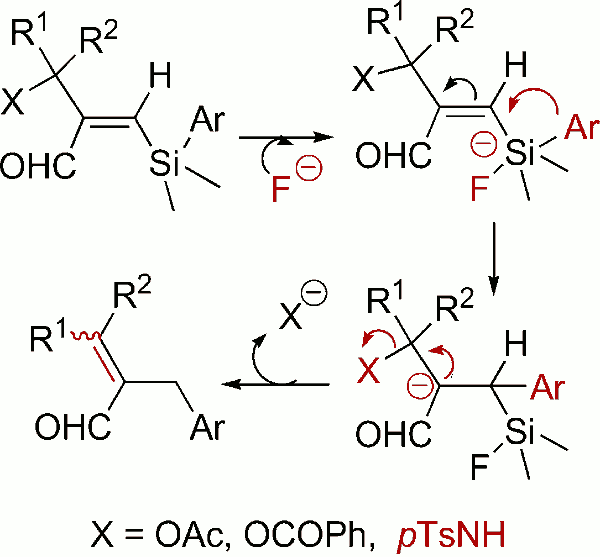
\includegraphics[width=1\textwidth]{img/substrati/ammine-desilil2.png}}\end{figure}
\end{columns}

\end{frame}

\subsubsection{Sililcarbociclizzazione}\begin{frame}\frametitle{Ammine propargiliche}\framesubtitle{Sililcarbociclizzazione}
In presenza di una {\bf base forte} (è stata impiegata una base organica ingombrata: DBU (1,8-Diazabiciclo[5.4.0]undec-7-ene)) {\bf la sililformilazione porta alla formazione di $\beta$-lattami}. 

Sembra che la base sia necessaria per spezzare il legame N--H.
\begin{figure}{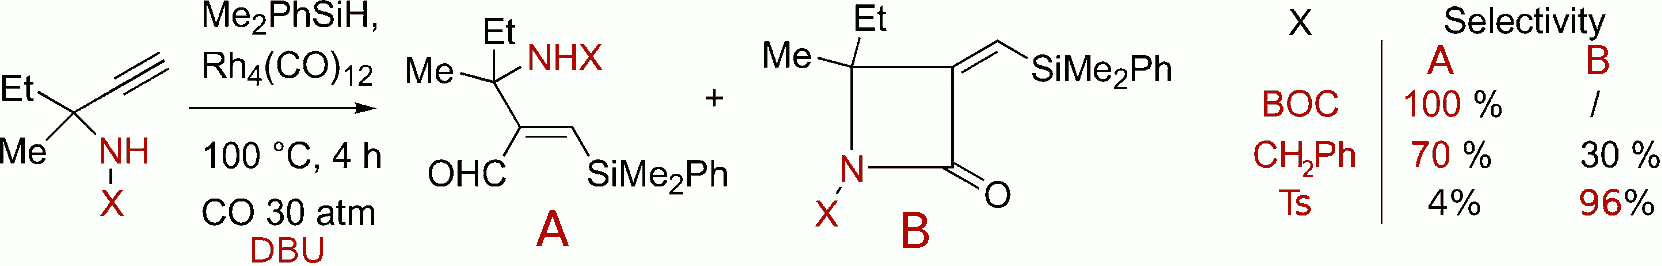
\includegraphics[width=1\textwidth]{img/substrati/ammine-cicliz.png}}\end{figure}
\pause
Contrariamente alla sililformilazione (favorita da alchini non ramificati) la {\bf sililcarbociclizzazione avviene bene solo se impiegata su alchini completamente sostituiti in posizione propargilica}.

\end{frame}

%%%%%%%%%%%%%%%%%%%%%%%%%%%%%%%%%%%%%%%%%%%%%%%%%%%%%%%%%%%%%%%%%%%%
\logo{}
\subsubsection{Desililazione di $\alpha$-sililmetilene $\beta$-lattami}\begin{frame}\frametitle{Ammine propargiliche}\framesubtitle{Desililazione di $\alpha$-sililmetilene $\beta$-lattami}
\begin{columns}
\column{0.6\linewidth}
Su $\alpha$-sililmetilene $\beta$-lattami la {\bf desililazione} con migrazione del gruppo aromatico avviene con {\bf buone rese} in 3-metilaril-$\beta$-lattame e alte diastereoselettività a favore del prodotto E più stabile.

\column{0.4\linewidth}
\vskip -13pt
\begin{figure}{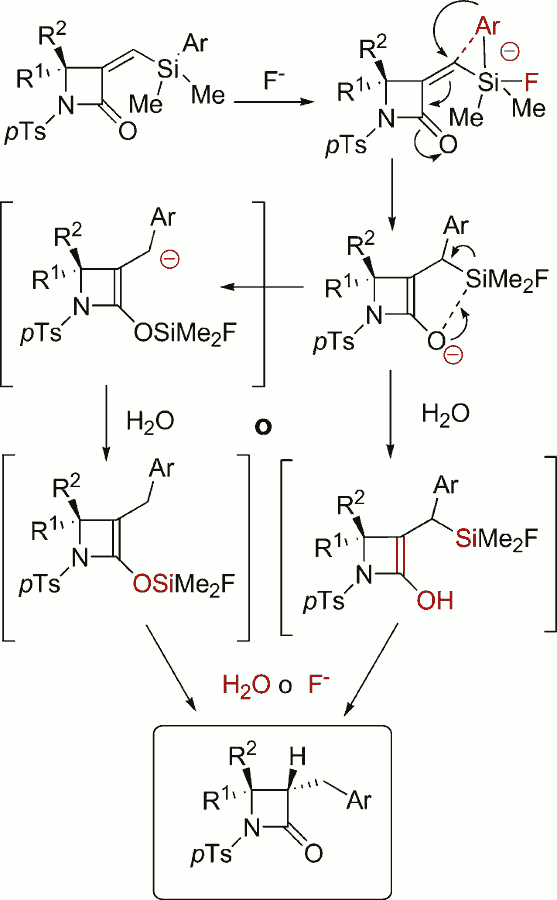
\includegraphics[width=1\textwidth]{img/substrati/ammine-cicl-desilil.png}}\end{figure}
\end{columns}
 
\end{frame}

\logo{
\includegraphics[width=0.07\paperwidth]{img/snslogo.png}}

%%%%%%%%%%%%%%%%%%%%%%%%%%%%%%%%%%%%%%%%%%%%%%%%%%%%%%%%%%%%%%%%%%%%
\diapo{Estensioni}
Una reattività simile alle ammine propargiliche si ottiene trattando alcoli propargilici ed omopropargilici:

 è possibile ottenere $\beta$ e $\gamma$ lattoni aventi in posizione 3 dei metilarili.
\begin{figure}{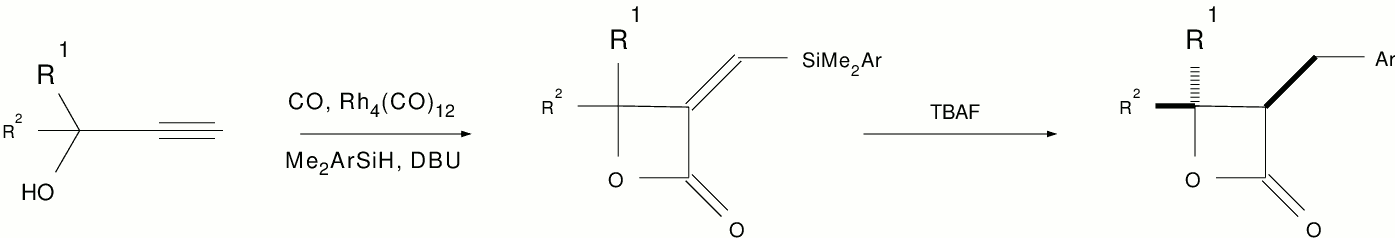
\includegraphics[width=1\textwidth]{img/substrati/alcol-tutto.png}}\end{figure}

     \end{frame}

%%%%%%%%%%%%%%%%%%%%%%%%%%%%%%%%%%%%%%%%%%%%%%%%%%%%%%%%%%%%%%%%%%%%

\subsection{Appendice: Alcoli propargilici}
\subsubsection{Sililformilazione}\begin{frame}\frametitle{Alcoli propargilici}\framesubtitle{Sililformilazione}
La {\bf sililformilazione di alcoli propargilici} in assenza di base avviene con {\bf buone rese}. 

A differenza delle precedenti sililformilazioni si ottengono diastereoselettività minori a causa della produzione del prodotto E in quantità dal 4 al 20\%. 
\begin{figure}{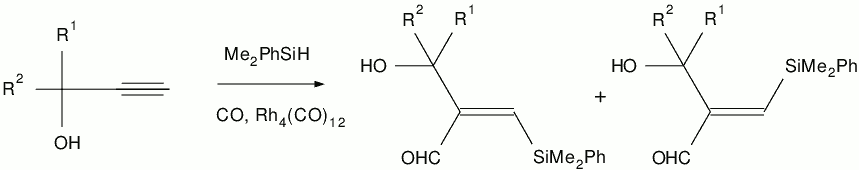
\includegraphics[width=0.9\textwidth]{img/substrati/alcol-sililform.png}}\end{figure}

\end{frame}
\logo{}
%%%%%%%%%%%%%%%%%%%%%%%%%%%%%%%%%%%%%%%%%%%%%%%%%%%%%%%%%%%%%%%%%%%%
\subsubsection{Desililazione di $\beta$-sililalchenali}\begin{frame}\frametitle{Alcoli propargilici}\framesubtitle{Desililazione di $\beta$-sililalchenali}
\begin{columns}
\column{0.5\linewidth}
Durante la {\bf desililazione} indotta da fluoruri si ha {\bf eliminazione} del gruppo OH alcolico.

Questo diviene un buon gruppo uscente a causa dell'alta affinità con il silicio.
\column{0.5\linewidth}
\begin{figure}{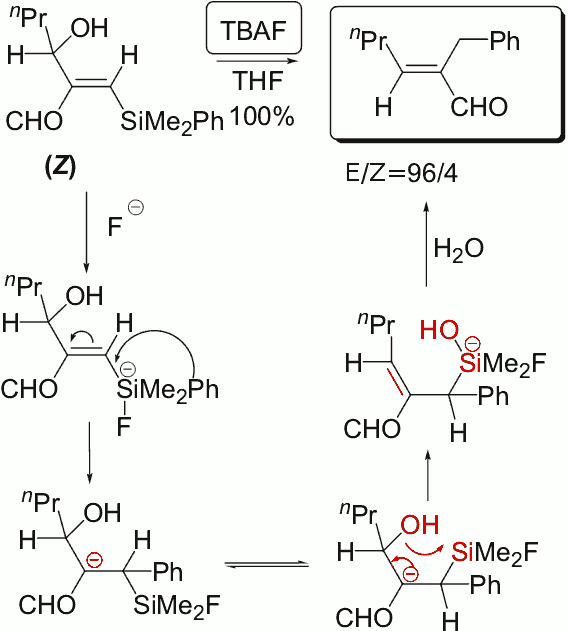
\includegraphics[width=1\textwidth]{img/substrati/alcol-desilil.png}}\end{figure}
     \end{columns}     
  \end{frame}\logo{
\includegraphics[width=0.07\paperwidth]{img/snslogo.png}}

\subsubsection{Sililcarbociclizzazione}\begin{frame}\frametitle{Alcoli propargilici}\framesubtitle{Sililcarbociclizzazione}
Nella {\bf sililformilazione di alcoli} propargilici in presenza di base DBU si ottengono rese in $\beta$-lattoni dipendenti dal substrato:
\begin{itemize}
 \item su alcoli propargilici {\bf primari} si ottiene solo {\bf sililformilazione};
 \item su alcoli {\bf secondari} si ottiene una {\bf miscela} di prodotti (a meno di usare sul silano aromatici ingombrati in orto);
\begin{figure}{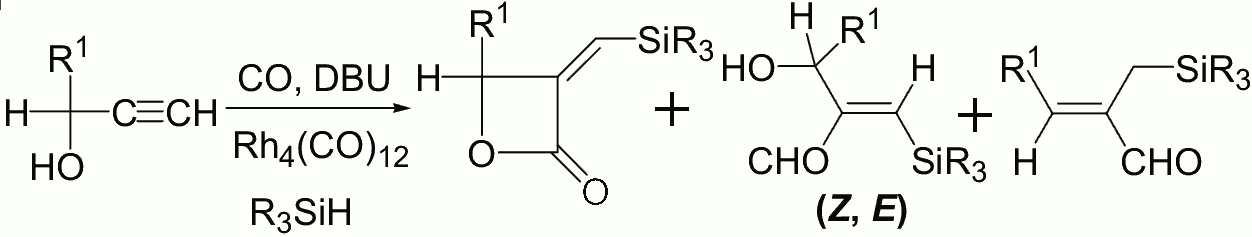
\includegraphics[width=0.7\textwidth]{img/substrati/alcol-secondari.png}}\end{figure}
 \item su alcoli {\bf terziari} alifatici si hanno {\bf buone rese} in $\beta$ lattoni;
 \item sul 2-fenil-3-butin-2-olo si hanno miscele di prodotti (alle alte temperature di reazione il lattone decompone con perdita di \ce{CO2}, a temperature più basse di può ottenere il lattone).
\end{itemize}
\end{frame}



%%%%%%%%%%%%%%%%%%%%%%%%%%%%%%%%%%%%%%%%%%%%%%%%%%%%%%%%%%%%%%%%%%%%
\subsubsection{Desililazione di $\alpha$-sililmetilene $\beta$-lattoni}\begin{frame}\frametitle{Alcoli propargilici}\framesubtitle{Desililazione di $\alpha$-sililmetilene $\beta$-lattoni}
                                                             La {\bf desililazione} con migrazione del gruppo aromatico {\bf procede bene con ogni lattone} trattato (tranne il 3-benzil-4-fenil-4-metil-ossetan-2-one che aveva già dato problemi di decomposizione nella sililcarbociclizzazione).

La desililazione è risultata altamente {\bf diastereoselettiva} permettendo di ottenere prodotti con i sostituenti più ingombranti in trans.
\begin{figure}{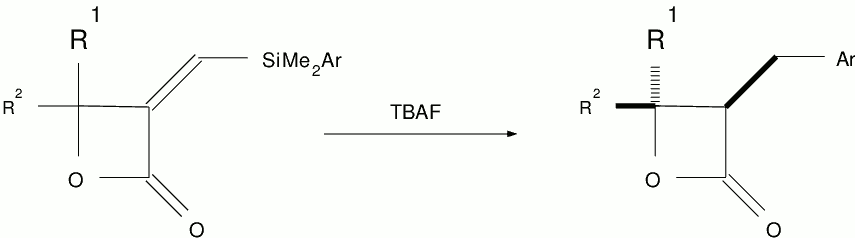
\includegraphics[width=0.85\textwidth]{img/substrati/alcol-desililcicl.png}}\end{figure}
\end{frame}



\nocite{*}
\begin{frame}[shrink]
\bibliographystyle{plainnat}
\bibliography{colloquio4.bib}
\end{frame}

\end{document}
